\documentclass[11pt]{article}
\usepackage[margin=1in]{geometry}
\usepackage{amsmath}
\usepackage[version=4]{mhchem}
\usepackage[T1]{fontenc}
\usepackage{lmodern}
\usepackage[authoryear,round]{natbib}
\usepackage{graphicx}
\usepackage{float}
\usepackage{booktabs}
\usepackage{array}
\usepackage{indentfirst}

\title{Supporting Information: Event-Timing Tests and Sensitivity Analyses}
\author{}
\date{}

\begin{document}
\renewcommand{\thefigure}{S\arabic{figure}}
\renewcommand{\thetable}{S\arabic{table}}
\maketitle

\section*{Supporting Information}

\subsection*{Text S1. Orbital phase assignment and Rayleigh tests}

We converted the precession index and obliquity into circular phase variables using their local extrema. After removing adjacent extrema of the same type so that minima and maxima alternated, minima were assigned phase \(0\), maxima phase \(\pi\), and the unwrapped phase was linearly interpolated between extrema before wrapping to \([0,2\pi)\). Under this convention, precession-index minima correspond to \(0^\circ\) and maxima to \(180^\circ\). Events requiring extrapolation beyond the available extrema were excluded from the corresponding Rayleigh test.

For each event type and orbital driver, we applied the Rayleigh test for non-uniformity on the circle following standard circular-statistics methods \citep{mardia2000directional}. Given event phases \(\theta_j\), the resultant vector is
\[
\mathbf{R} =
\left(
\sum_{j=1}^{n}\cos\theta_j,\,
\sum_{j=1}^{n}\sin\theta_j
\right),
\]
and the mean resultant length is
\[
\bar{R} = \frac{\|\mathbf{R}\|}{n}.
\]
The mean phase is \(\arg(\mathbf{R})\), and the Rayleigh statistic is
\[
z = n\bar{R}^{2}.
\]
We used the standard finite-sample correction for the Rayleigh \(p\) value. A significant result indicates departure from circular uniformity but does not adjust for event history, sampling resolution, or slow background-state covariates.

The main text reports the significant precession-phase clustering. Obliquity phases do not show comparable clustering: \(p=0.682\) for strong starts and \(p=0.704\) for weak starts. One weak-start event required obliquity-phase extrapolation and was excluded, giving \(n=99\) for that test. The obliquity Rayleigh tests and phase-ECDF diagnostics are shown in Figures~\ref{fig:obliquity_rayleigh} and \ref{fig:phase_ecdf_uniform_check}.


\subsection*{Text S2. Bin-width and history-window sensitivity}

Repeating the precession-phase comparison for 0.2--1.0 kyr bins preserved the result after event history, sampling resolution, LR04, and \(\ce{CO2}\) were included. Empty-bin fractions decreased from approximately 97\% at 0.2 kyr to approximately 85\% at 1.0 kyr, but all bin-width variants retained significant and closely aligned phase responses.

We also varied the same-type event-history window used in the event-process baseline. Repeating the analysis for \(W=1\), 2, 5, and 10 kyr preserved the phase result. The reported \(p\) values are likelihood-ratio tests for adding precession phase after the climate-state model, and the preferred phases are from the corresponding full predictive models. For strong starts, \(p=2.2\times10^{-5}\)--\(1.6\times10^{-4}\) and preferred phases were \(2.0^\circ\)--\(8.1^\circ\). For weak starts, \(p=4.5\times10^{-4}\)--\(2.1\times10^{-3}\) and preferred phases were \(227.7^\circ\)--\(238.4^\circ\). 

\subsection*{Text S3. Composite age-uncertainty sensitivity}

Because a full ensemble of Cheng et al. (2016) composite age models is not available here, we used a simple age-dependent uncertainty envelope. The assumed two-sigma uncertainty increases exponentially from 1 kyr at 0 kyr BP to 7.4 kyr at 640 kyr BP, intentionally conservative relative to typical U--Th errors in the younger part of the record. This envelope was interpolated to each Rousseau et al. (2023) 0.4--4 kyr KS-window start age, and one standard deviation was taken as one half of the two-sigma value.

We generated 500 age-randomized catalogues for each transition type. Perturbed ages were drawn from the corresponding Gaussian distribution and truncated by adjacent-event midpoint bounds and by the 0--640 kyr BP analysis interval. Each randomized catalogue therefore retained the observed event count and rank order while allowing individual ages to vary within the prescribed uncertainty envelope.

For each randomized catalogue, we repeated the Rayleigh precession test, the test for adding precession phase after the climate-state model, and the full-predictive-model test against the event-process baseline. Perturbation magnitudes and significance fractions are shown in Figure~\ref{fig:age_uncertainty_sensitivity}; the main robustness values are reported in the main text.


\subsection*{Text S4. Lagged predictive-information diagnostics}

The lagged predictive-information scan is a temporal-alignment diagnostic, not a causal-delay estimator. The best single-driver lags are reported in the main text. Their corresponding maximum gains are 0.108, 0.124, and 0.127 bits/event for LR04, \(\ce{CO2}\), and precession phase in the strong-start catalogue, and 0.111, 0.158, and 0.068 bits/event in the weak-start catalogue. The weak-start single-driver precession scan has nominal \(p=0.010\) at its best lag but is not significant after false-discovery-rate correction.

Conditional scans give the same near-zero phase result. After LR04 and \(\ce{CO2}\) are fixed at their best single-driver lags, precession phase peaks at 0 kyr for both strong starts (0.141 bits/event, \(p=1.16\times10^{-4}\)) and weak starts (0.108 bits/event, \(p=7.12\times10^{-4}\)); both remain significant after false-discovery-rate correction. When LR04, \(\ce{CO2}\), and precession phase share the same lag, the best precession lag is 0 kyr for strong starts and 0.8 kyr for weak starts. These maxima indicate contemporaneous orbital-phase organization in this binned framework, not a resolved causal response time.

\subsection*{Text S5. Sparse-bin and bootstrap likelihood diagnostics}

The 0.2 kyr event bins are intentionally sparse. This sparsity does not by itself imply zero inflation: for an event rate of approximately 0.03 events per bin, a Poisson process predicts about 97\% empty bins. In the full predictive model, observed and expected empty-bin fractions are 0.9701 and 0.9708 for strong starts, and 0.9691 and 0.9699 for weak starts. Pearson dispersion estimates are 0.872 and 0.916, respectively. Thus, the main fitted models do not show evidence for excess zeros or overdispersion.

We also checked the two central nested likelihood-ratio tests using reduced-model parametric bootstrap null distributions. For each bootstrap replicate, event catalogues were simulated under the fitted reduced model, same-type event history was recomputed from the simulated catalogue, and both reduced and full models were refitted. This dynamic-history bootstrap preserves the serial dependence induced by the overlapping 5 kyr history windows, rather than treating \(H_i\) as a fixed independent covariate. We used 2000 bootstrap replicates for each event type and comparison; all refits converged. The empirical \(p\) value was computed as
\[
p_{\mathrm{boot}}=
\frac{1+\#\{\mathrm{LR}^{(b)}\geq \mathrm{LR}_{\mathrm{obs}}\}}
{1+B},
\]
with \(B=2000\). The bootstrap distributions are slightly heavier-tailed than the asymptotic \(\chi^2\) reference, but all four central comparisons remain significant (Table~\ref{tab:bootstrap_lrt_diagnostics}).

\subsection*{Text S6. Barker et al. D-O warming catalogue sensitivity}

We used the variable-threshold D-O warming catalogue of \citet{barker2011800} as an independent event-catalogue sensitivity test. These events are not monsoon transitions and do not provide a weak-start analogue, so they are used only as a one-sided check on transitions toward warmer Greenland/interstadial-like conditions. This test is independent of both the Cheng et al. speleothem composite and the Rousseau et al. KS detection workflow.

We analyzed three variants: the European Project for Ice Coring in Antarctica Dome C 3 (EDC3) age scale over 0--800 kyr, EDC3 ages cropped to 0--640 kyr, and SpeleoAge over 0--400 kyr. For each, we repeated the Rayleigh test and the nested predictive-information models used in the main analysis. The event-process baseline contained 5 kyr same-type event history and a sampling-resolution term. Resolution was estimated from local EPICA Dome C age spacing; for SpeleoAge, bin centers were first mapped to EDC3 age using the Barker supplementary age mapping. The EDC3 0--640 kyr inputs and fitted event rates are shown in Figure~\ref{fig:barker_inputs_rates}.

The Barker Rayleigh tests do not reject uniform precession phase: \(\bar{R}=0.135\), \(p=0.151\) for EDC3 0--640 kyr; \(\bar{R}=0.118\), \(p=0.177\) for EDC3 0--800 kyr; and \(\bar{R}=0.189\), \(p=0.081\) for SpeleoAge 0--400 kyr. Thus, this independent catalogue does not reproduce the direct circular clustering seen in the Rousseau speleothem catalogue, although the SpeleoAge subset is marginal.

The predictive-information tests nevertheless show a Barker analogue of the two-step structure in the main analysis (Figure~\ref{fig:barker_predictive_sensitivity}). LR04+\(\ce{CO2}\) improves prediction after the EDC event-process baseline in all three variants: \(\mathrm{LR}=8.33\), \(p=0.0155\), \(\Delta\mathrm{AICc}=-4.32\), and 0.0583 bits/event for EDC3 0--640 kyr; \(\mathrm{LR}=11.32\), \(p=0.00348\), \(\Delta\mathrm{AICc}=-7.31\), and 0.0653 bits/event for EDC3 0--800 kyr; and \(\mathrm{LR}=8.87\), \(p=0.0118\), \(\Delta\mathrm{AICc}=-4.85\), and 0.0927 bits/event for SpeleoAge 0--400 kyr.

Adding precession phase after the Barker climate-state model also improves all three variants: \(\mathrm{LR}=7.95\), \(p=0.0188\), \(\Delta\mathrm{AICc}=-3.94\), and 0.0557 bits/event for EDC3 0--640 kyr; \(\mathrm{LR}=6.80\), \(p=0.0334\), \(\Delta\mathrm{AICc}=-2.78\), and 0.0392 bits/event for EDC3 0--800 kyr; and \(\mathrm{LR}=7.74\), \(p=0.0209\), \(\Delta\mathrm{AICc}=-3.71\), and 0.0809 bits/event for SpeleoAge 0--400 kyr. These phase gains correspond to average per-event likelihood multipliers of 1.039, 1.028, and 1.058, respectively. We interpret this as support for conditional background-state and precession-phase information, not as an independent replication of the stronger Rayleigh phase-clustering result.

\clearpage
\section*{Tables}

\begin{table}[H]
\centering
\footnotesize
\caption{
Reduced-model parametric bootstrap likelihood-ratio diagnostics for the two central predictive-model comparisons.
The bootstrap regenerated event catalogues under the fitted reduced model, recomputed same-type event history, and refitted the reduced and full models for each replicate.
This preserves the serial dependence induced by overlapping 5 kyr history windows.
The empirical \(p\) value is \((1+\#\{\mathrm{LR}^{(b)}\geq\mathrm{LR}_{\mathrm{obs}}\})/(1+B)\), with \(B=2000\).
}
\label{tab:bootstrap_lrt_diagnostics}
\begin{tabular}{@{}>{\raggedright\arraybackslash}p{0.28\textwidth}
                >{\centering\arraybackslash}p{0.10\textwidth}
                >{\centering\arraybackslash}p{0.08\textwidth}
                >{\centering\arraybackslash}p{0.11\textwidth}
                >{\centering\arraybackslash}p{0.11\textwidth}
                >{\centering\arraybackslash}p{0.09\textwidth}@{}}
\toprule
Comparison & Event & LR & \(\chi^2\) \(p\) & Bootstrap \(p\) & Exceed. \\
\midrule
Climate-state model vs. event-process baseline & Strong & 13.73 & 0.00104 & 0.00250 & 4/2000 \\
Climate-state model vs. event-process baseline & Weak & 21.69 & \(1.95\times10^{-5}\) & 0.00050 & 0/2000 \\
Precession phase after climate-state model & Strong & 19.74 & \(5.16\times10^{-5}\) & 0.00050 & 0/2000 \\
Precession phase after climate-state model & Weak & 14.52 & 0.00070 & 0.00200 & 3/2000 \\
\bottomrule
\end{tabular}
\end{table}

\begin{table}[H]
\centering
\small
\caption{Sensitivity of the core phase and predictive-information tests to the Rousseau et al. KS detection-window choice. Values are p-values for the complete 0.4--4 kyr and 0.6--4 kyr transition catalogues. Asterisks indicate \(p < 0.05\). The ``Consistent'' column indicates that the same significance decision (\(p<0.05\) or \(p\geq0.05\)) is reached for both KS window choices.}
\label{tab:ks_window_core_sensitivity}
\begin{tabular}{>{\raggedright\arraybackslash}p{0.14\textwidth}
                >{\raggedright\arraybackslash}p{0.37\textwidth}
                >{\centering\arraybackslash}p{0.12\textwidth}
                >{\centering\arraybackslash}p{0.12\textwidth}
                >{\centering\arraybackslash}p{0.10\textwidth}}
\toprule
Event catalogue & Test & KS 0.4--4 kyr & KS 0.6--4 kyr & Consistent \\
\midrule
Strong starts & Rayleigh precession phase & 0.0019* & 0.0010* & Yes \\
Strong starts & Climate-state model vs. event-process baseline & 0.0010* & 0.0017* & Yes \\
Strong starts & Precession phase after climate-state model & $5.16\times10^{-5}$* & $8.76\times10^{-6}$* & Yes \\
Strong starts & LR04 unique in full predictive model & 0.0716 & 0.0466* & No \\
Strong starts & CO$_2$ unique in full predictive model & 0.332 & 0.403 & Yes \\
Strong starts & Full predictive model vs. event-process baseline & $9.54\times10^{-7}$* & $2.79\times10^{-7}$* & Yes \\
\midrule
Weak starts & Rayleigh precession phase & 0.0027* & 0.0012* & Yes \\
Weak starts & Climate-state model vs. event-process baseline & $1.95\times10^{-5}$* & 0.00040* & Yes \\
Weak starts & Precession phase after climate-state model & 0.00070* & 0.00031* & Yes \\
Weak starts & LR04 unique in full predictive model & 0.665 & 0.904 & Yes \\
Weak starts & CO$_2$ unique in full predictive model & 0.0118* & 0.0218* & Yes \\
Weak starts & Full predictive model vs. event-process baseline & $2.62\times10^{-7}$* & $2.13\times10^{-6}$* & Yes \\
\bottomrule
\end{tabular}
\end{table}

\clearpage
\section*{Figures}

\begin{figure}[H]
    \centering
    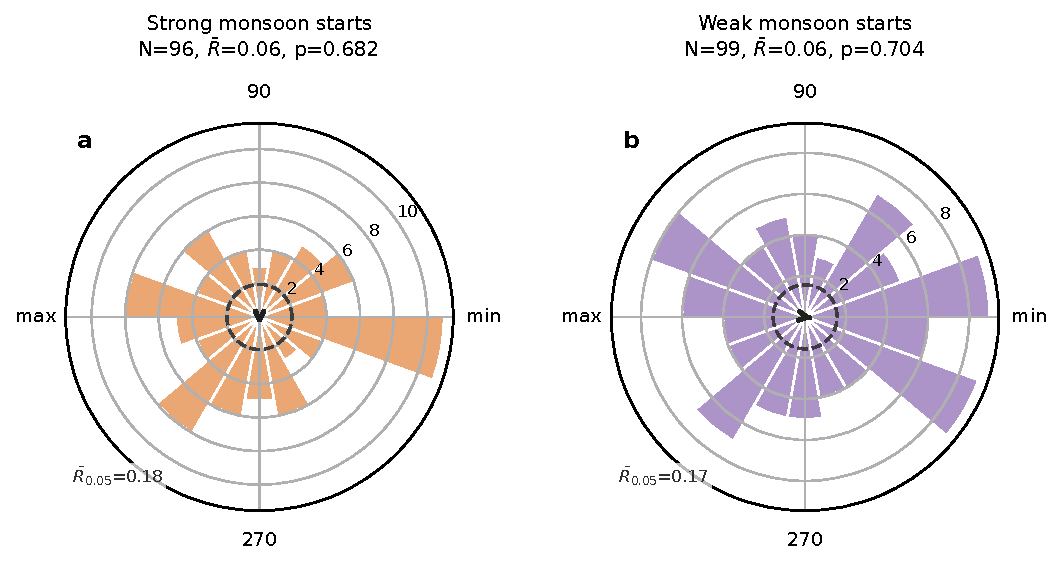
\includegraphics[width=1\textwidth]{figures/FigS01.pdf}
    \caption{Obliquity-phase Rayleigh tests.
    Rayleigh tests for clustering of strong and weak monsoon starts in obliquity phase; arrows show the mean resultant direction and dashed circles mark the $p=0.05$ threshold. Obliquity from \citet{laskar2004long}; event catalogue from \citet{rousseau2023reliable}.
    }
    \label{fig:obliquity_rayleigh}
\end{figure}

\begin{figure}[H]
    \centering
    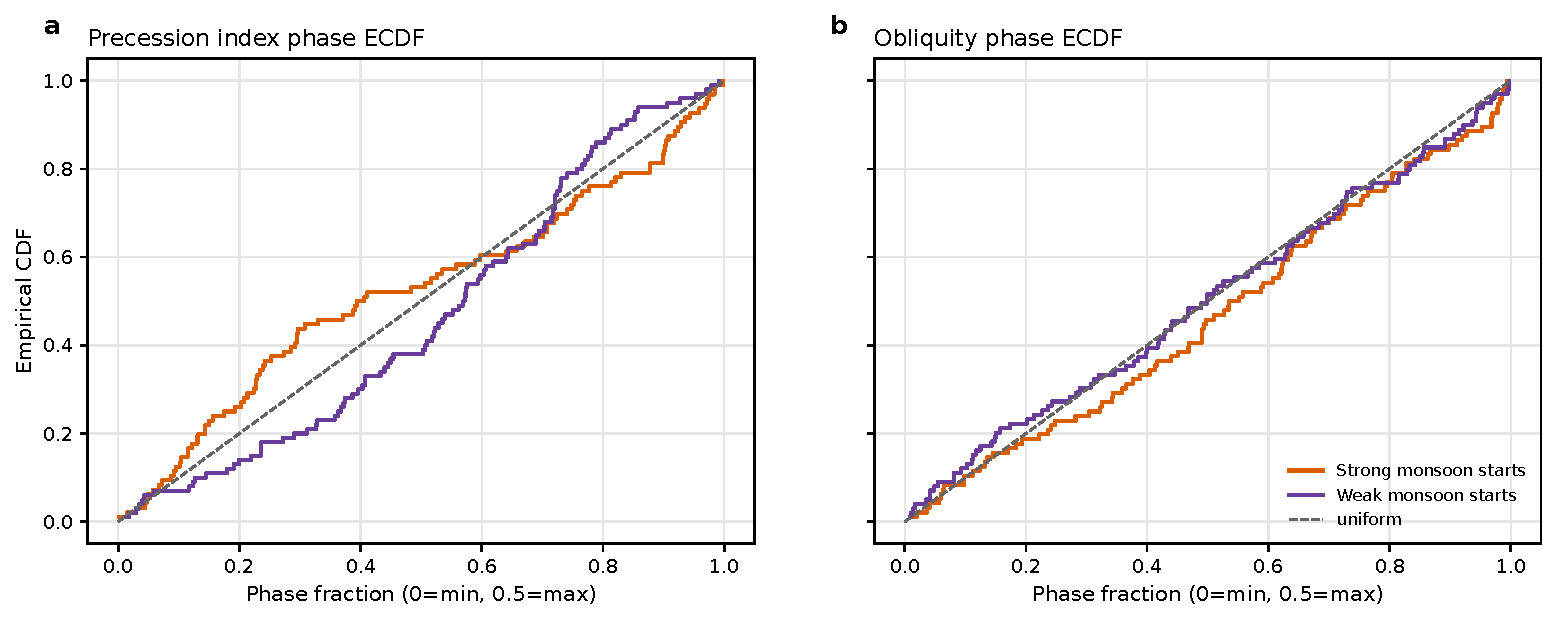
\includegraphics[width=\textwidth]{figures/FigS02.pdf}
    \caption{
    Phase uniformity diagnostics.
    Empirical cumulative distributions of monsoon-start phases relative to
    (a) the precession index~\citep{laskar2004long} and (b) obliquity~\citep{laskar2004long}.
    Phase fraction 0 denotes an orbital-series minimum, 0.5 denotes a maximum,
    and 1 denotes the next minimum.
    The dashed line shows the expectation for uniformly distributed phases.
    Curves close to the dashed line indicate no preferred phase, whereas
    systematic departures indicate phase clustering. Strong and weak monsoon
    starts show clear departures from uniformity for precession phase but remain
    close to uniform for obliquity.
    }
    \label{fig:phase_ecdf_uniform_check}
\end{figure}

\begin{figure}[H]
    \centering
    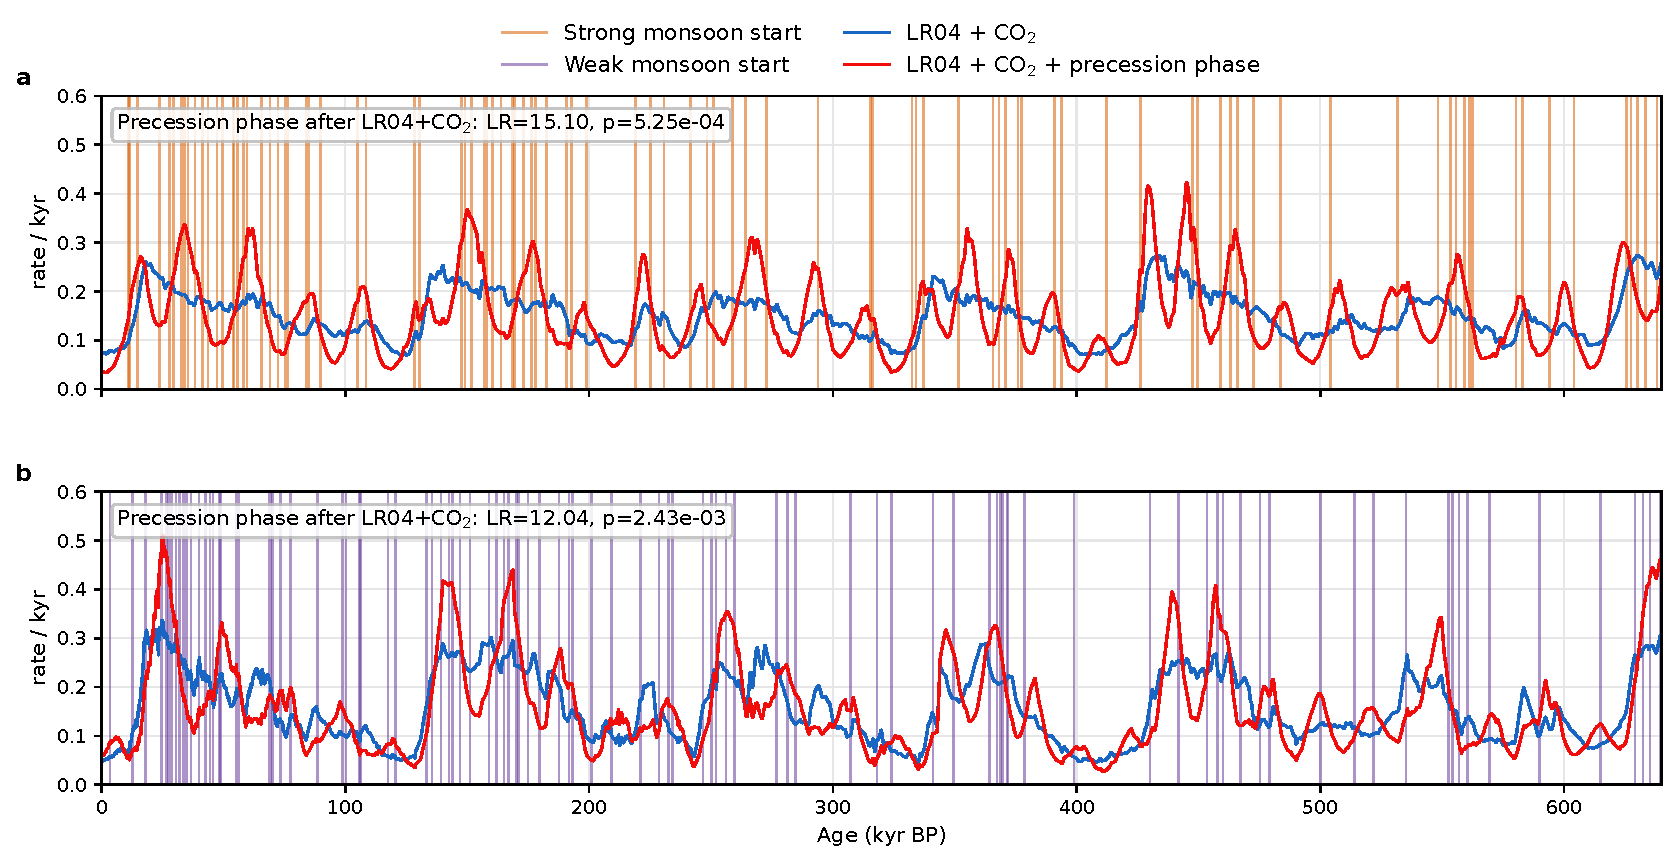
\includegraphics[width=1\textwidth]{figures/FigS03.pdf}
    \caption{
    Climate-state and precession-phase fitted event rates without event-process controls.
    Fitted binned Poisson event rates from the LR04+\(\ce{CO2}\) model and the LR04+\(\ce{CO2}\)+precession-phase model are shown for (a) strong and (b) weak monsoon starts.
    Vertical lines mark observed event bins.
    This visualization omits same-type event history and sampling-resolution controls, so it is not the main reference model; it is included to show the slower climate-state rate modulation and the superposed precession-phase structure more clearly.
    Text boxes report likelihood-ratio tests for adding the two precession-phase terms to the LR04+\(\ce{CO2}\) model.
    LR04, \(\ce{CO2}\), and precession phase are from \citet{lisiecki2005pliocene}, \citet{bereiter2015revision}, and \citet{laskar2004long}, respectively.
    }
    \label{fig:climate_phase_hazards_no_event_baseline}
\end{figure}

\begin{figure}[H]
    \centering
    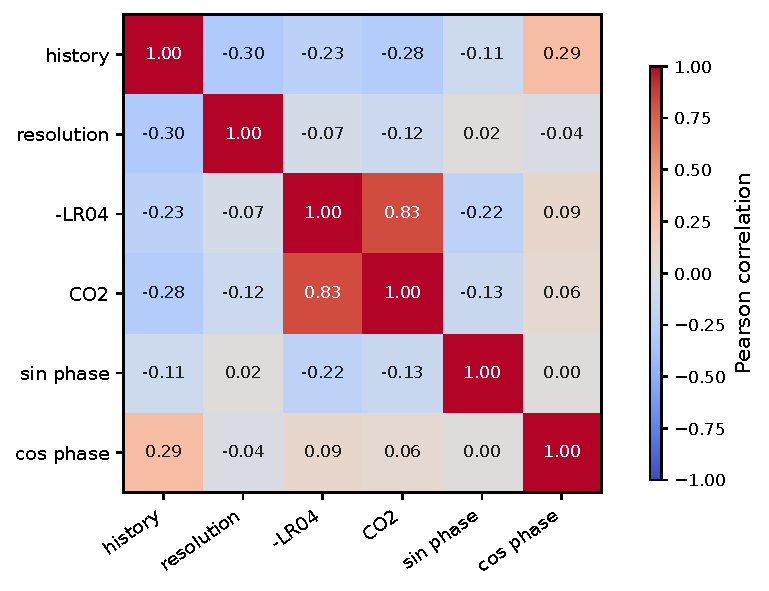
\includegraphics[width=0.68\textwidth]{figures/FigS04.pdf}
    \caption{
    Extended-baseline predictor correlations.
    Correlations among predictors in the extended baseline, defined as the full predictive model used as the reference for additional-forcing sensitivity tests.
    The matrix includes same-type event history, Cheng composite sampling resolution~\citep{cheng2016asian}, $-$LR04~\citep{lisiecki2005pliocene}, \(\ce{CO2}\)~\citep{bereiter2015revision}, and the sine and cosine terms used to represent precession phase~\citep{laskar2004long}.
    LR04 is sign-inverted only for display, so its correlation with \(\ce{CO2}\) is positive; the fitted models use the original LR04 orientation.
    The strong correlation between $-{}$LR04 and \(\ce{CO2}\) is consistent with treating them as partly overlapping indicators of slow glacial background state.
    Precession-phase terms are only weakly correlated with the event-process and background-state controls.
    }
    \label{fig:extended_baseline_correlation}
\end{figure}

\begin{figure}[H]
    \centering
    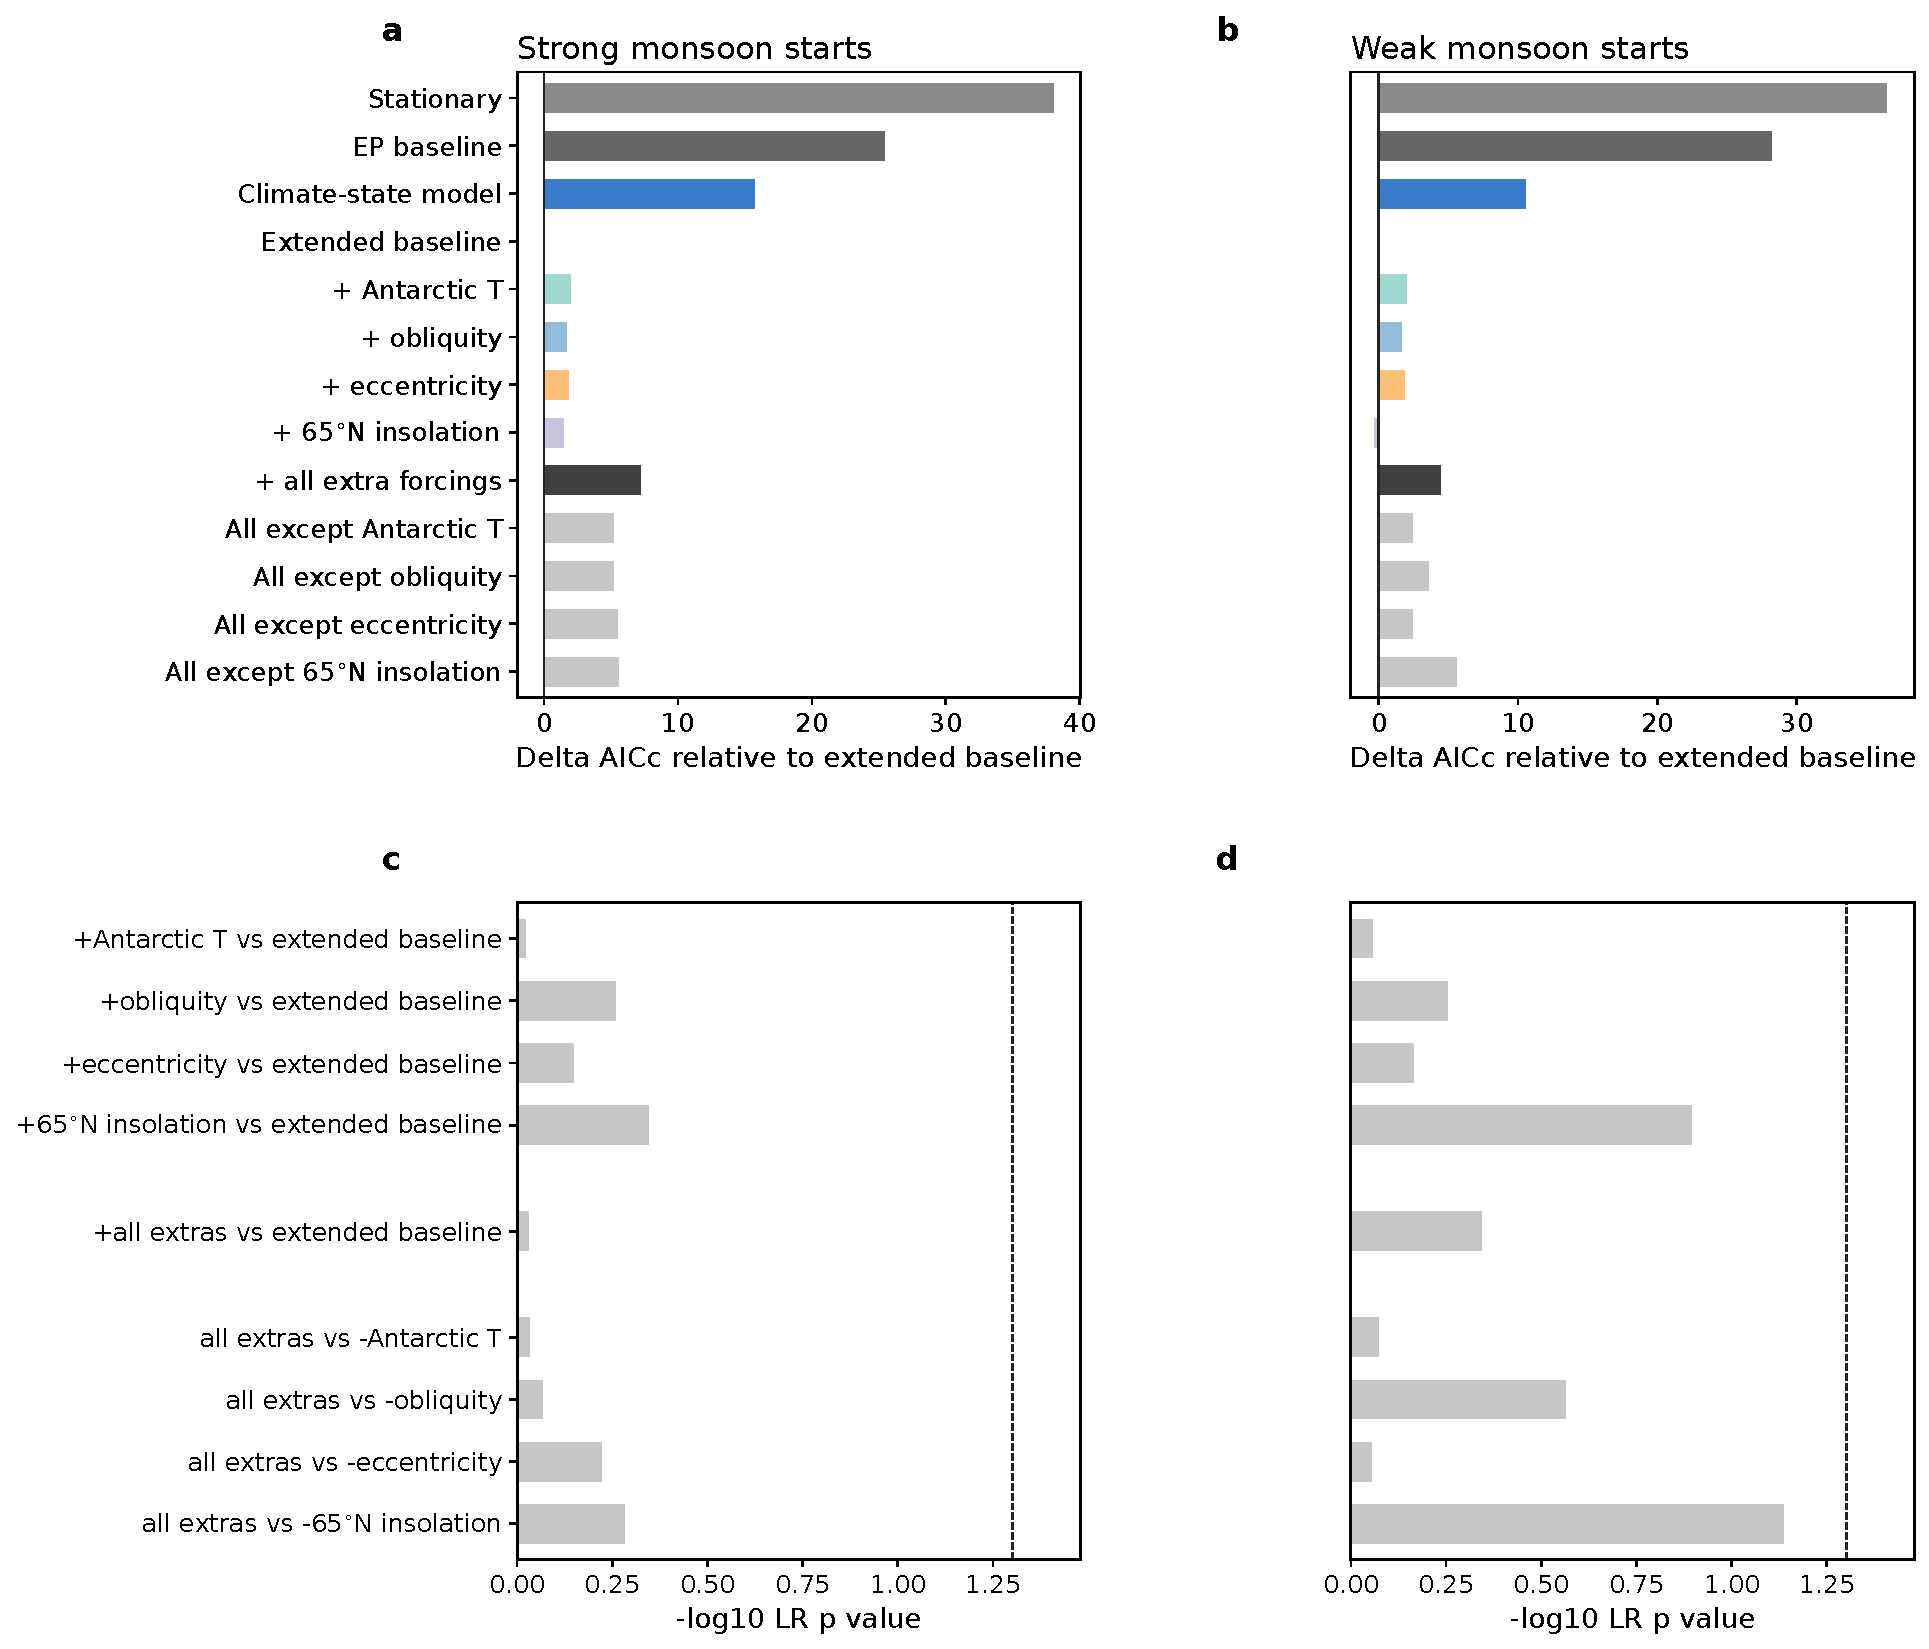
\includegraphics[width=1\textwidth]{figures/FigS05.pdf}
    \caption{
    Additional-forcing sensitivity.
    Sensitivity of predictive-information models to additional forcings.
    (a,b) \(\Delta\)AICc for strong and weak monsoon starts, measured relative to the extended baseline, i.e., the full predictive model before adding extra forcings.
    In (a,b), labels beginning with \(+\) add the listed forcing or forcings to the extended baseline, whereas ``All except \(X\)'' denotes the all-extra model with \(X\) omitted.
    (c,d) Nested likelihood-ratio tests for the extra forcings. Bars show \(-\log_{10}(p)\), and the dashed line marks \(p=0.05\); bars to the left of this line are not significant.
    Labels of the form ``\(+X\) vs extended baseline'' compare the extended baseline+\(X\) model with the extended baseline, and labels of the form ``all extras vs \(-X\)'' compare the all-extra model with a reduced model omitting \(X\).
    }
    \label{fig:sensitivity_aicc_lrt}
\end{figure}

\begin{figure}[H]
    \centering
    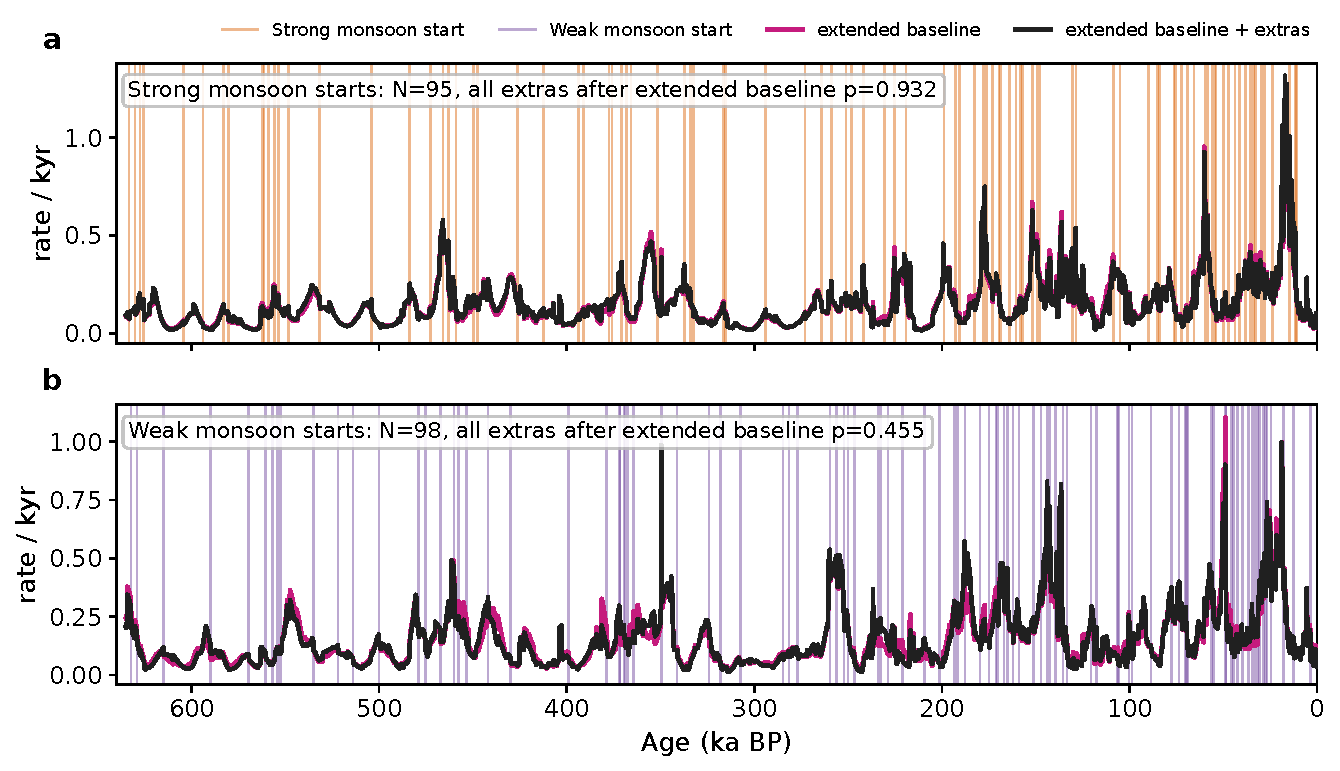
\includegraphics[width=1\textwidth]{figures/FigS06.pdf}
    \caption{
    Extended-forcing fitted event rates.
    Fitted event rates from the predictive-information models are shown for (a) strong and (b) weak monsoon starts.
    Vertical lines mark observed event bins.
    Magenta curves show the extended baseline, i.e., the full predictive model before adding extra forcings;
    black curves show the extended model after adding Antarctic temperature,
    obliquity, eccentricity, and 65$^\circ$N summer-solstice insolation.
    The similar fitted rates and nonsignificant likelihood-ratio tests indicate
    that the extra forcings do not significantly improve the extended baseline.
    }
    \label{fig:base_vs_extended_hazards}
\end{figure}

\begin{figure}[H]
    \centering
    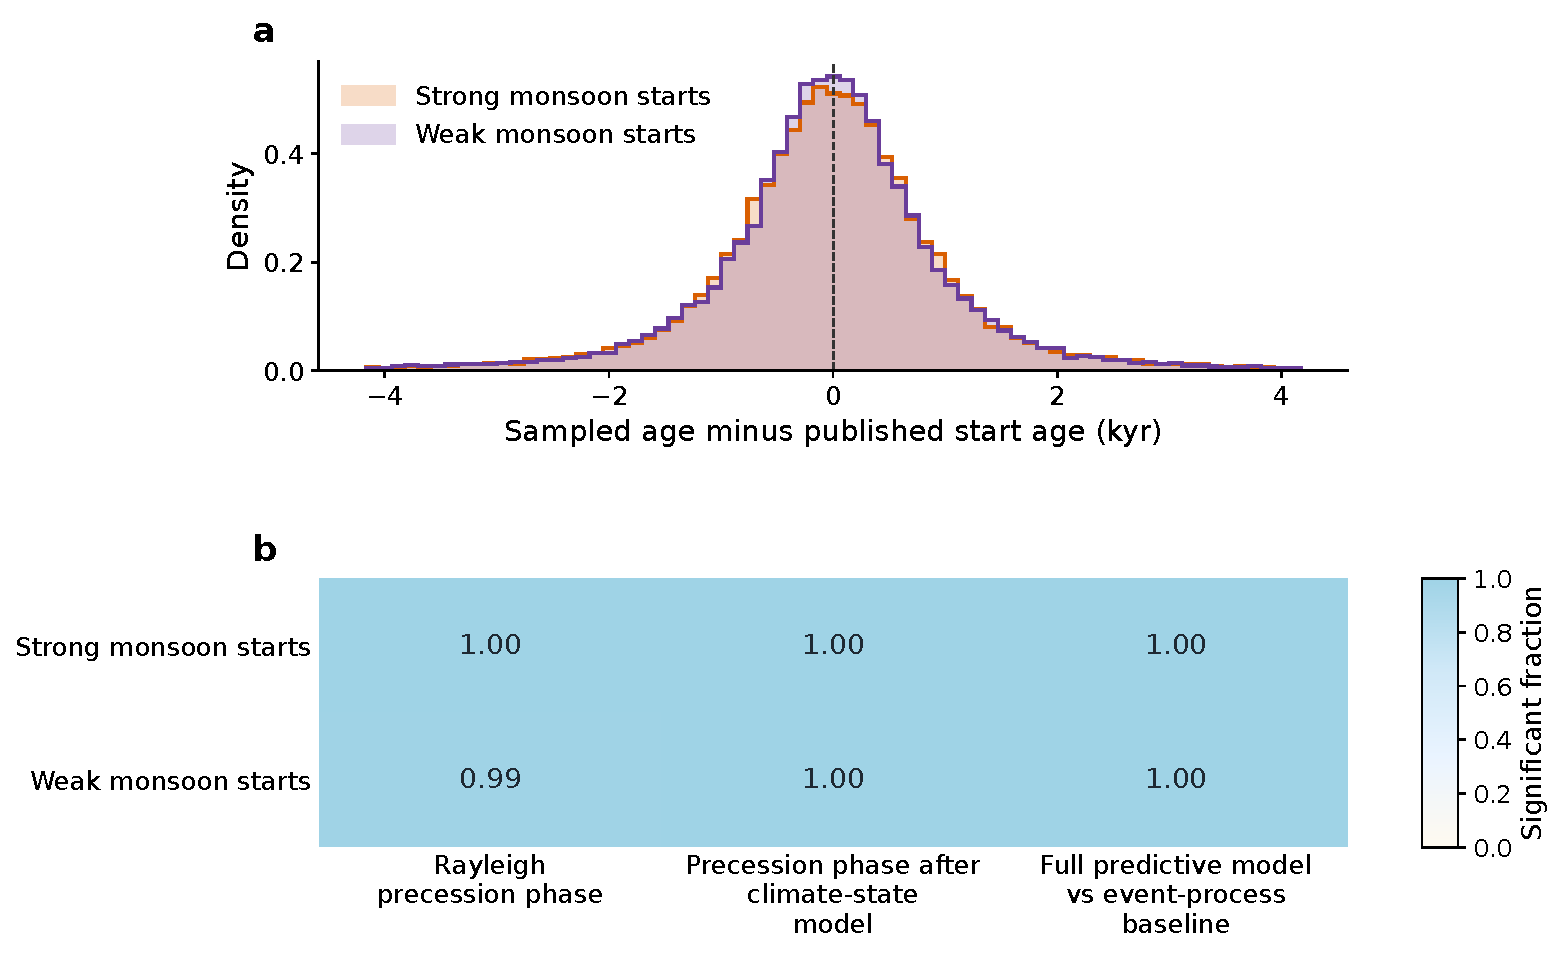
\includegraphics[width=0.85\linewidth]{figures/FigS07.pdf}
    \caption{Composite-age uncertainty sensitivity.
    (a) Distribution of age perturbations applied to the published Rousseau et al.~\citep{rousseau2023reliable} 0.4--4 kyr KS-window strong and weak monsoon-start ages, after rank-preserving truncation.
    (b) Fraction of 500 age-randomized catalogues for which each test remains significant at \(p<0.05\).
    Precession-phase clustering and predictive-information results remain significant for nearly all or all randomized catalogues.}
    \label{fig:age_uncertainty_sensitivity}
\end{figure}

\begin{figure}[H]
    \centering
    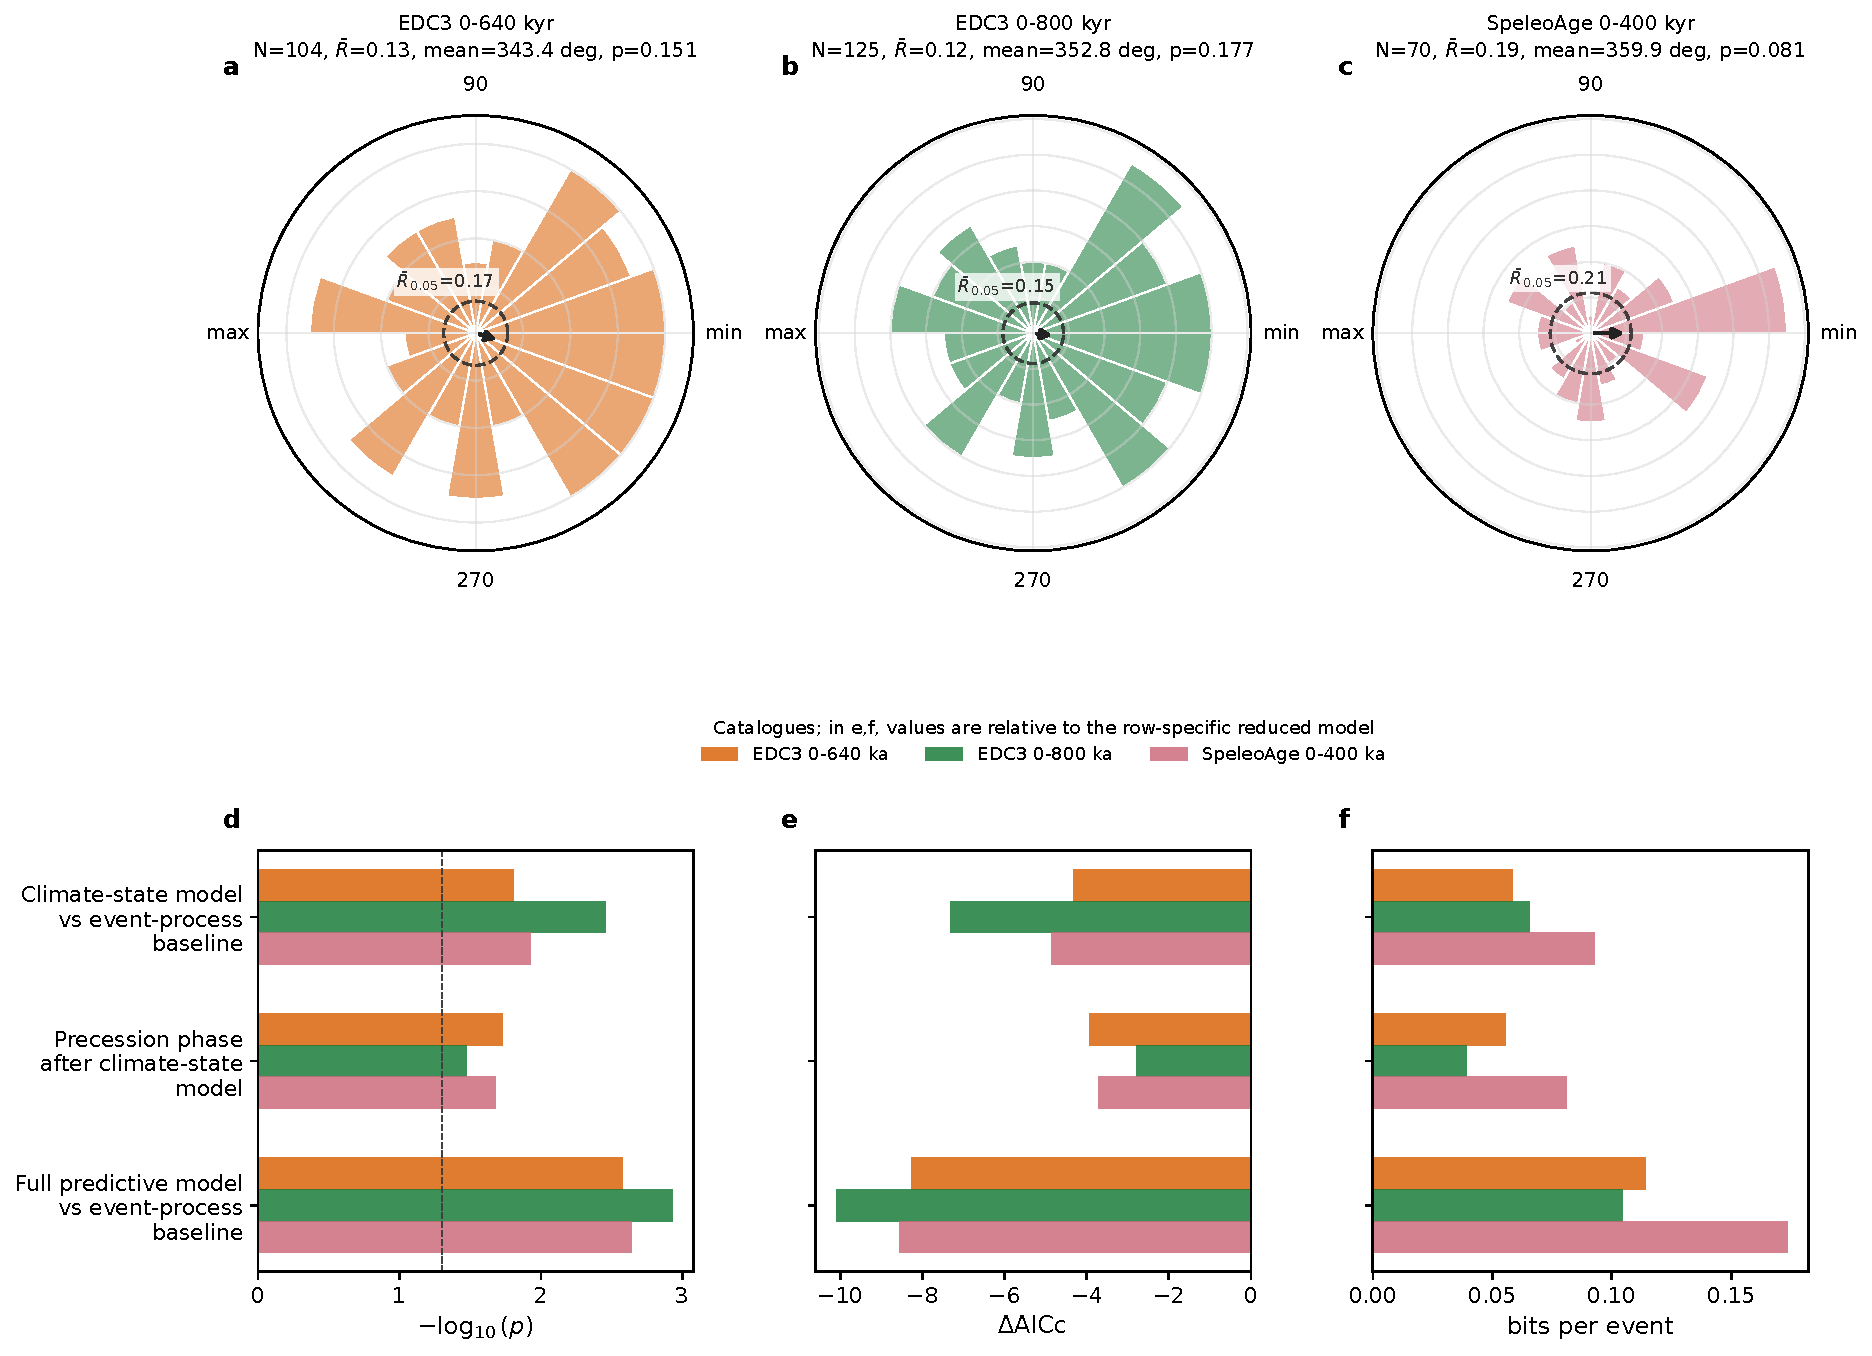
\includegraphics[width=1\textwidth]{figures/FigS08.pdf}
    \caption{
    Barker et al. D-O warming catalogue sensitivity.
    (a--c) Precession-phase Rayleigh tests for the \citet{barker2011800} variable-threshold D-O warming catalogue under three age/support choices; arrows show the mean resultant direction and dashed circles mark the \(p=0.05\) threshold.
    (d) Nested likelihood-ratio tests shown as \(-\log_{10}(p)\); the dashed line marks \(p=0.05\).
    (e) \(\Delta\)AICc, defined as full minus reduced model for each row; negative values favour the fuller model.
    (f) Predictive-information gain in bits per event for the same full-versus-reduced comparison.
    Labels are full-model versus reduced-model comparisons; ``Full predictive model vs climate-state'' denotes adding precession phase to the Barker climate-state model.
    }
    \label{fig:barker_predictive_sensitivity}
\end{figure}

\begin{figure}[H]
    \centering
    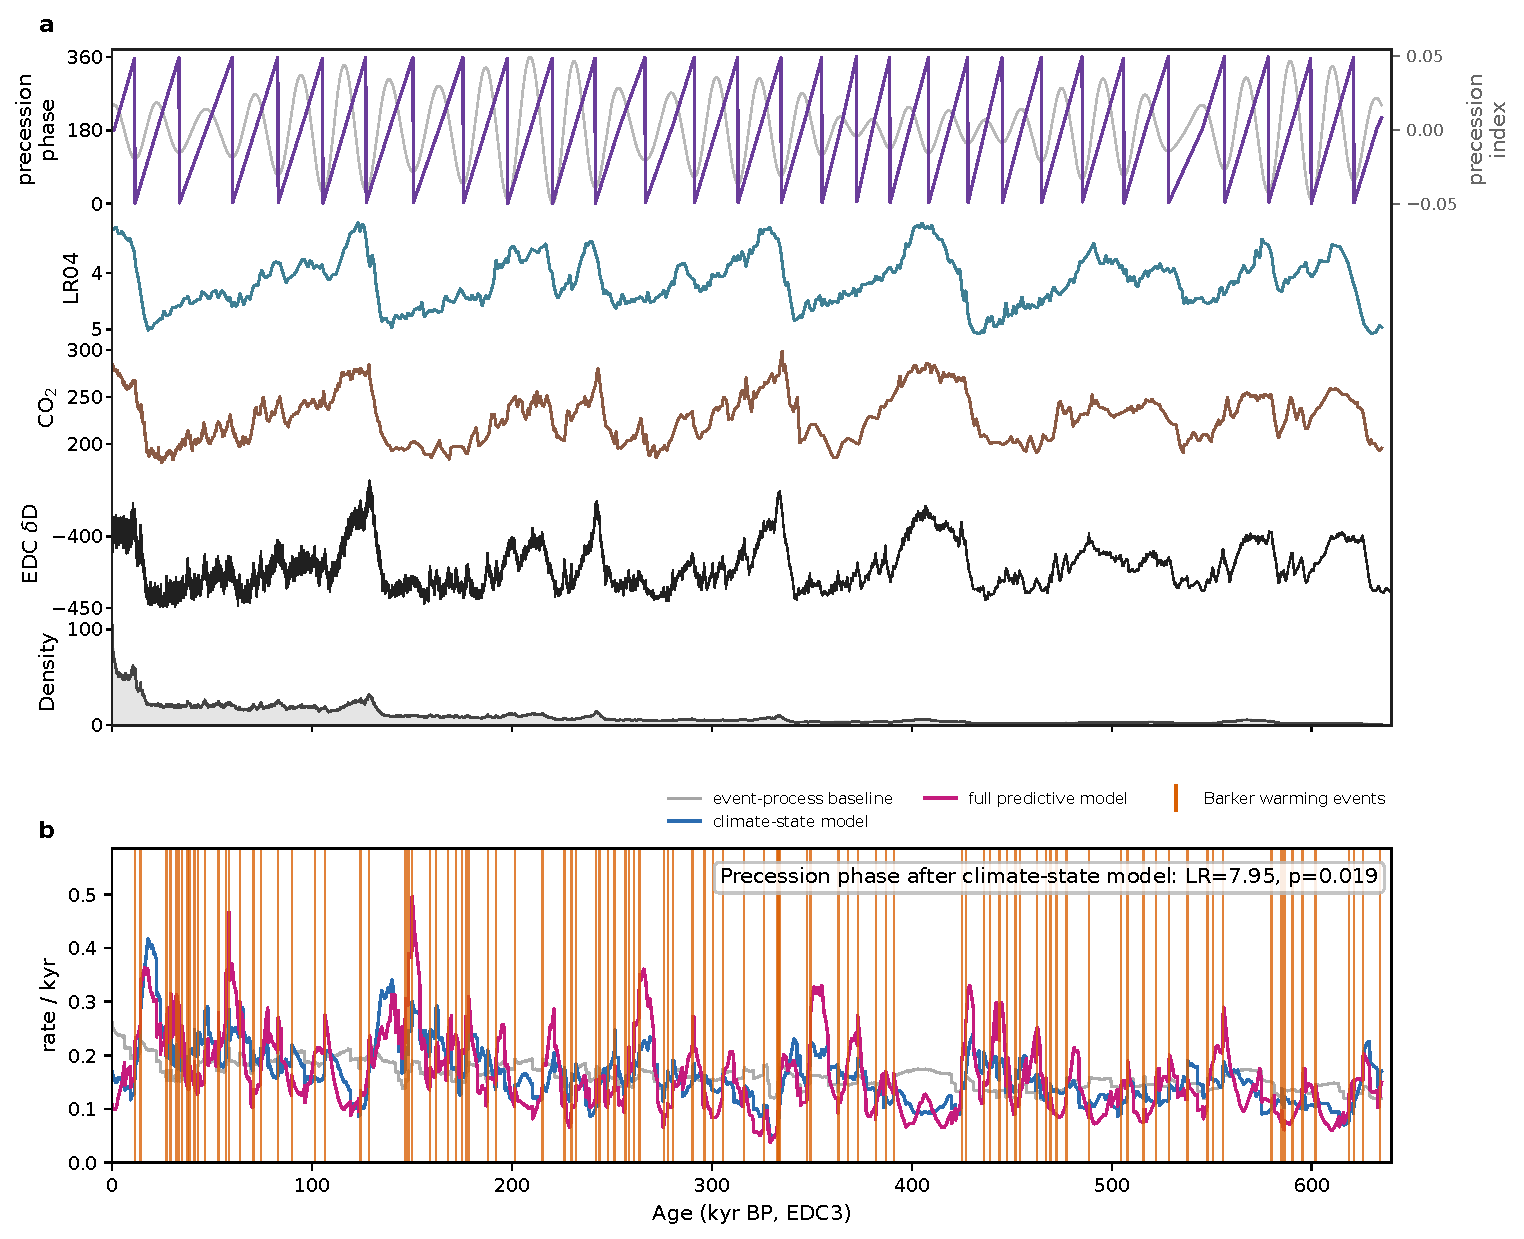
\includegraphics[width=1\textwidth]{figures/FigS09.pdf}
    \caption{
    Barker EDC3 0--640 kyr inputs and fitted event rates.
    (a) Stacked input series: precession phase and raw precession index~\citep{laskar2004long}, LR04~\citep{lisiecki2005pliocene}, atmospheric \(\ce{CO2}\)~\citep{bereiter2015revision}, EDC \(\delta\)D~\citep{jouzel2007orbital}, and local EDC sampling density estimated from the EDC record used for the sampling-resolution term.
    (b) Fitted Barker warming-event rates for the event-process baseline, climate-state model, and full predictive model; vertical lines mark Barker variable-threshold warming events.
    }
    \label{fig:barker_inputs_rates}
\end{figure}

\bibliographystyle{agu}
\bibliography{reference}
\end{document}
